\usetikzlibrary{arrows.meta}
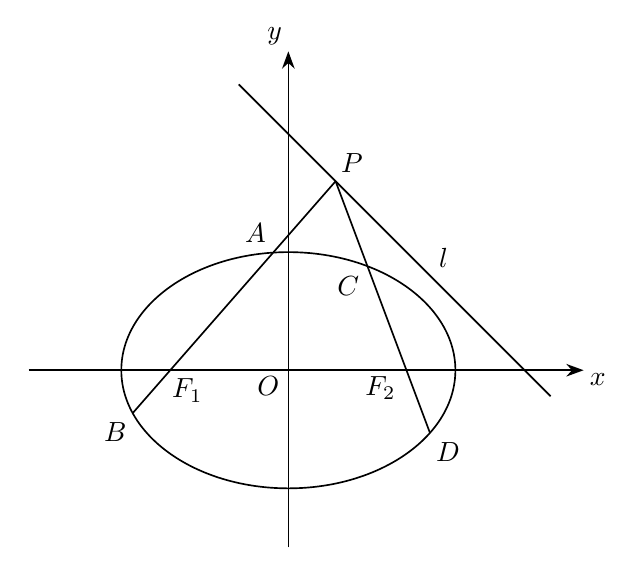
\begin{tikzpicture}[x=1.5cm,y=1.5cm,line width=.6pt,>={Stealth[length=2.2mm,width=1.6mm]},font=\normalsize]
  \draw[->] (-2.2,0)--(2.5,0);
  \draw[->] (0,-1.5)--(0,2.7);
  \draw (0,0) ellipse [x radius=1.41421356, y radius=1];
  \draw (-0.42,2.42)--(2.22,-0.22);
  \draw (0.4,1.6)--(-1.31770,-0.36309);
  \draw (0.4,1.6)--(1.19890,-0.53040);
  \node[anchor=north west,inner sep=0pt,xshift=2pt,yshift=-1pt] at (2.5,0) {$x$};
  \node[anchor=south east,inner sep=0pt,xshift=-2pt,yshift=2pt] at (0,2.7) {$y$};
  \node[anchor=north east,inner sep=0pt,xshift=-3pt,yshift=-2pt] at (0,0) {$O$};
  \node[anchor=north west,inner sep=0pt,yshift=-2pt] at (-0.99,-0.02) {$F_1$};
  \node[anchor=north,inner sep=0pt,yshift=-2pt] at (0.78,0) {$F_2$};
  \node[anchor=south west,inner sep=0pt,xshift=0pt,yshift=1pt] at (0.44,1.64) {$P$};
  \node[anchor=south east,inner sep=0pt,xshift=-1pt,yshift=1pt] at (-0.16,1.05) {$A$};
  \node[anchor=north east,inner sep=0pt,xshift=-1pt,yshift=-1pt] at (-1.34,-0.41) {$B$};
  \node[anchor=north east,inner sep=0pt,xshift=-1pt,yshift=-1pt] at (0.63,0.82) {$C$};
  \node[anchor=north west,inner sep=0pt,xshift=1pt,yshift=-1pt] at (1.22,-0.58) {$D$};
  \node[anchor=south west,inner sep=0pt,xshift=0pt,yshift=1pt] at (1.27,0.84) {$l$};
\end{tikzpicture}
